\documentclass[]{article}

% Imported Packages
%------------------------------------------------------------------------------
\usepackage{amssymb}
\usepackage{amstext}
\usepackage{amsthm}
\usepackage{amsmath}
\usepackage{enumerate}
\usepackage{fancyhdr}
\usepackage[margin=1in]{geometry}
\usepackage{graphicx}
\usepackage{float}
%\usepackage{extarrows}
%\usepackage{setspace}
%------------------------------------------------------------------------------

% Header and Footer
%------------------------------------------------------------------------------
\pagestyle{plain}  
\renewcommand\headrulewidth{0.4pt}                                      
\renewcommand\footrulewidth{0.4pt}                                    
%------------------------------------------------------------------------------

% Title Details
%------------------------------------------------------------------------------
\title{Deliverable \#2}
\author{SE 3A04: Software Design II -- Large System Design}
\date{}                               
%------------------------------------------------------------------------------

% Document
%------------------------------------------------------------------------------
\begin{document}

\maketitle	
\noindent{\bf Tutorial Number:} T01\\
{\bf Group Number:} G6 \\
{\bf Group Members:} 
\begin{itemize}
	\item Jane Klavir
	\item Nathan Luong
	\item Areez Visram
	\item Jennifer Ye
\end{itemize}

\section{Introduction}
\label{sec:introduction}
% Begin Section

The following document is dedicated to applying the requirements listed in the SRS in a practical manner to identify design details of the system. It will go into specifics on a class-level, demonstrating what the forecasted classes should be, and how they should interact with one-another within subsystems as well as the overall program architecture. This app is meant to be a long-term project for the company, meaning this document has the possibility of changing in the future.

\subsection{Purpose}
\label{sub:purpose}
% Begin SubSection
This document dives into the design of the system, describing the precise classes and system architecture. Accordingly, this document is largely meant for app developers, to give them a good idea of the framework of the program, and how various components interact with one another. Thus, reading this document will provide a comprehensive picture on the way the system is constructed.
% End SubSection

\subsection{System Description}
\label{sub:system_description}
% Begin SubSection
Our system is organized in such a way that the overall pattern follows the Model-View-Controller (MVC) architecture. Using this style is practical for our system given that there are several data models (e.g. users, rides, prompts), controllers that carry out the logic of the system (e.g. UserController and RidesController), and the necessity for a highly interactive UI. Our system requires constant data processing, which is anticipated for highly dynamic systems such as taxi networks. There is also frequent interaction between users with other users, as well as users with the system, and our architecture organizes the system components in a coordinated way.\\\\
The system also has a couple of subsystems. The dispatcher is essentially the match-maker between the carpoolers. It is primarily organized around the TaxiSessionController, and interacts with a number of other classes, and follows a repository architecture. Then, the user profile subsystem handles the group of classes that manage user data, such as RegistrationController, CustomerEditPage, and other classes in that sphere. The other subsystems are the GPS, which interfaces with Google Maps for all navigation and location-tracking purposes, and the prompt generator, which implements an in-taxi game for carpoolers.

% End SubSection

\subsection{Overview}
\label{sub:overview}
% Begin SubSection
The rest of this document goes into further details on what has been described. In particular, Section 2 includes an analysis class diagram, which identifies the classes in our program, categorizes them, and exhibits their relationships with one another. Section 3 provides an overview of the structural design of the application; it identifies the specific architectural styles used for both the system as a whole, and subsystems. Section 4 comprises the Class Responsibility Collaboration (CRC) Cards, which identify the responsibilities and collaborators of each class in the program. Ultimately, this document applies the SRS to synthesize the requirements into a feasible design.

\subsection{References}
Qian, K. (2010). Software architecture and design illuminated. Jones and Bartlett Publ. 
% End SubSection

% End Section

\section{Analysis Class Diagram}
\label{sec:analysis_class_diagram}
% Begin Section
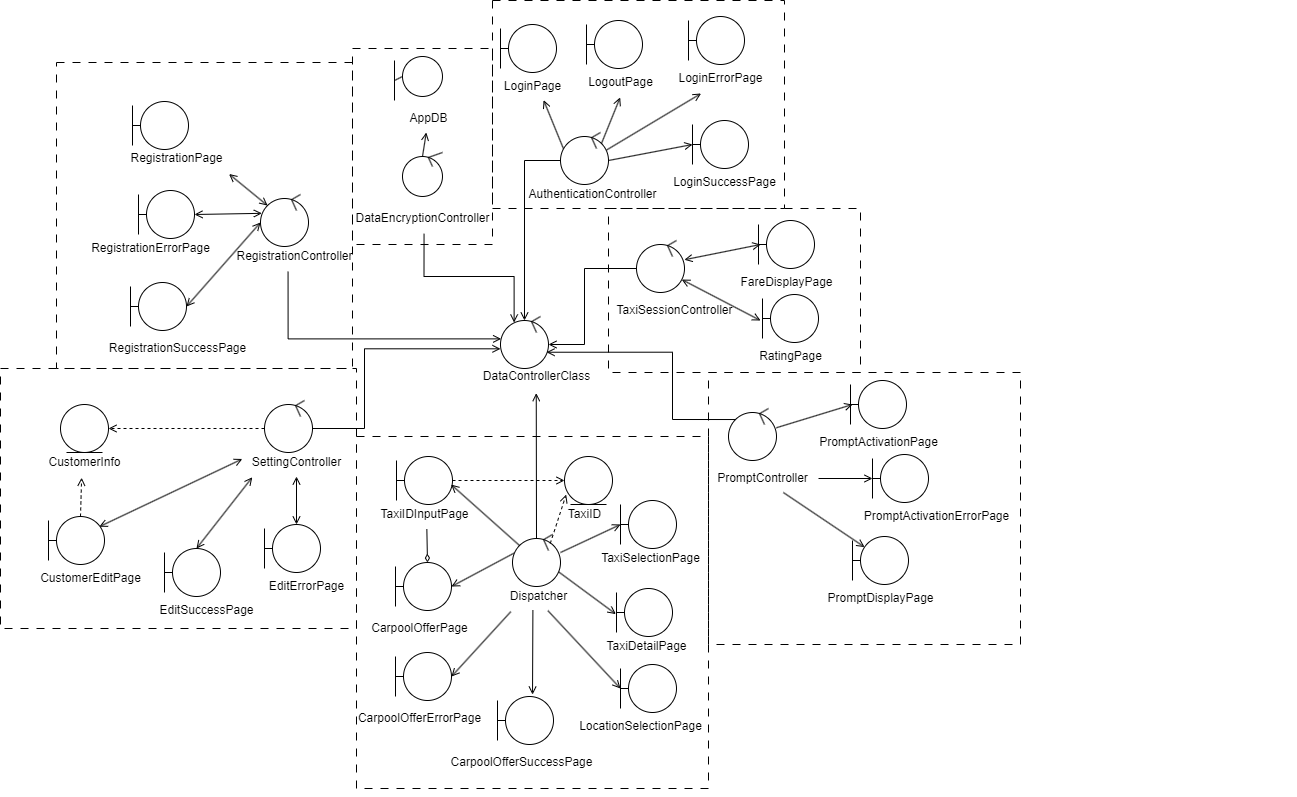
\includegraphics[scale = 0.45]{Graphics/ACD.png}

% End Section


\section{Architectural Design}
\label{sec:architectural_design}
% Begin Section

\subsection{System Architecture}
\label{sub:system_architecture}
% Begin SubSection
\subsubsection{Overall Architecture and Justification}
\label{subsub:overall_architecture}
% Begin SubSubSection
The overall architecture of the system is the Model-View-Controller (MVC) architecture, which is an interaction 
oriented architecture (Qian, 2010). The MVC architecture is the architecture that best fits the system that we are designing. The MVC style is best suited for 
interactive applications which contain multiple views for various data models (Qian, 2010). The application being implemented is heavily focused on the UI 
on the mobile app, and so an architecture style that allows for easy display of data into a UI view is suitable. Furthermore, our system contains multiple data models, for example, models for Users, 
Rides, Prompts and multiple pages/views across the application will interact with these data models. Furthermore, the MVC architecture is suitable for 
applications which are prone to frequent data changes (Qian, 2010). Our system is most definitely prone to frequent data changes, as rides are constantly being offered, 
arriving, and starting, which means the Rides model will be constantly updated and written to. Finally, the MVC architecture will allow us to separate the 
various logic functions into separate controllers. The architecture will allow for clear division of logic between controllers, which will make it easier 
to extend and modify the system. For example, we would have a UserController to handle user operations, a RidesController to handle ride operations and various 
other controllers to control the logic of other parts of the application. Given these benefits and the functionality of the system, we have chosen to implement 
the MVC architecture style for the main system.

\subsubsection{Subsystem Architectures and Justification}
Another architecture style will also be used for the various subsystems of our application. One of the subsystems within the main system is the Dispatcher 
subsystem, which is responsible for storing all information on taxis and carpool offerings, as well as deciding how to match carpool offers with 
requests that come in. The repository architecture style is best suited for systems (in this case a subsystem) in which a central data store stores information 
and various agents communicate with it (Qian, 2010). This architecture style fits the Dispatcher subsystem because the Dispatcher will contain a central data store which 
will store all the information about carpools. The data store will be passive, it will be like a database which just stores information and can be read from. 
The various agents for the repository will be the users who are requesting and offering carpools. These agents are active, as they drive the flow of the 
subsystem by sending carpool requests and offering carpools. The agents do not communicate directly with each other, they communicate via the data store by 
sending requests to the data store, and the data store facilitates the requests and decides appropriate matches. Given this, the repository architecture style 
is the most suitable for the Dispatcher subsystem.
% End SubSubSection

% Begin SubSubSection
\subsubsection{Structural Architecture Diagram}
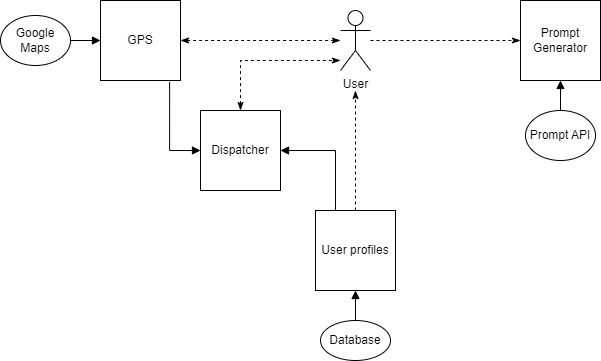
\includegraphics[scale = 0.7]{Graphics/subsystems_diagram_3.1.png}
% End SubSubSection

% Begin SubSubSection
\subsubsection{Design Alternatives Considered}
One design alternative for the main architecture that was considered was the Repository architectural style, which is a data centered architecture. We envisioned the system having a 
central passive database repository, with multiple active agents communicating with the data store. The agents were envisioned to be the different parts of 
the system, such as a user agent, a rides agent, a prompts agent, and then a dispatcher, all which communicated with the central data store. However, this design 
was not chosen because the system that is being built is a single mobile application connected to a database. The system does not involve multiple agents which 
must communicate with a central data store. If there were multiple applications that needed to communicate, this architecture style would be more applicable. However, 
is is a single application and the different parts of it can be represented using controllers within the architecture rather than external agents, so this design 
was not chosen. \\

\noindent The second design alternative for the main architecture that was considered was the Presentation-Abstraction-Control (PAC) architecture, which is also 
an interaction oriented architecture. Both MVC (the architecture that was chosen) and PAC could work for this system, but we ultimately chose MVC over PAC for 
various reasons. PAC was not chosen because PAC is more useful in complex applications, which require a hierarchical layering of agents. Our system is not complex, 
it is a single application that communicates with a database. In PAC, the only communication that can occur is between agents, and in our system, we would not 
have enough agents to justify having communication only between them. This would only add complexity. Furthermore, PAC is more useful for concurrent systems, which 
our app does not need to be to fulfill its requirements. Finally, PAC is less publicized and less widely used, and so for a somewhat inexperienced development team, MVC 
is a better choice as there are more resources, information and examples available to help in the design.
% End SubSubSection
% End SubSection

\subsection{Subsystems}
\label{sub:subsystems}
% Begin SubSection
 Provide a list of your subsystems, with a brief description of each. Be sure to document its purpose and relationship to other subsystems.
\\\\\\\\
The first subsystem is the dispatcher. Essentially, the dispatcher is a data store for all communications within our system. The dispatcher has several purposes. The first is to store information about active taxis in the fleet. It also stores information about user offers and requests. Subsequently, the dispatcher suggests “offerers” to “requesters”, and once a “requester” requests to join the “offerer’s” taxi, the dispatcher must also display an updated fare to the “offerer” so that they can make an informed decision. This match-making process is another fundamental purpose of the dispatcher.
\\\\
The next subsystem is the user profile subsystem, that handles tasks having to do with the processing and storage of user profiles. One main purpose of this subsystem is to facilitate the registration of new users. It records their information and remembers it in a database. Furthermore, another purpose is to allow registered users to make updates to their profile. When users edit their profiles, the user profile subsystem must make the necessary updates to the database so that all the information is up to date. Additionally, this subsystem allows registered users to delete their profiles, thenceforth these profiles are removed from the database.
\\\\
Another subsystem is the GPS. The purpose of this subsystem is to allow users to track the route of their taxi. Also, it uses the carpoolers’ locations to determine distances between carpoolers. The GPS subsystem requires interfacing with Google Maps.
\\\\
The final subsystem is the prompt generator. This subsystem executes our additional innovative feature, which is allowing carpoolers to socialize through a series interesting prompts. The prompt generator must also implement an API to fulfill its purpose of coming up with prompts.
\\\\
The subsystems interact with one another when it comes to the match-making procedure described in the dispatcher subsystem. The dispatcher is at the centre of it all, and for it to perform its role, it uses the user profile and GPS subsystems to obtain critical information. First, the user profiles subsystem provides data on users’ social preferences, which helps the dispatcher predict user compatibility. Then, the GPS subsystem returns distances between the taxi and potential matches, which the dispatcher uses in showing trip conditions (estimated fare, time, and distance). Ultimately, this relationship is one in which the dispatcher is the central unit, and it uses the other subsystems to get the necessary parameters for its algorithm.
\\
% End SubSection

% End Section
	
\section{Class Responsibility Collaboration (CRC) Cards}
\label{sec:class_responsibility_collaboration_crc_cards}
% Begin Section
% DataControllerClass

\begin{table}[H]
	\centering
	\begin{tabular}{|p{6cm}|p{6cm}|}
	\hline 
		\multicolumn{2}{|l|}{\textbf{Class Name: DataControllerClass}} \\
	\hline
	\textbf{Responsibility:} & \textbf{Collaborators:} \\
	\hline 
	Handles request to save Taxi Session Data (prices, rating, etc.) from TaxiSessionController for authenticated users & TaxiSessionController, DataEncryptionController\\ \hline 
	Handles request to fetch, and save Authetication Data (UID, username, password, etc.) from AuthenticationController &AuthenticationController, DataEncryptionController\\ \hline 
	Handles request to fetch Prompt Data (prompts, preferences, promt histories, etc.) from PromptController for authenticated users &PromptController, DataEncryptionController\\ \hline 
	Handles request to fetch, edit, and save CarPool Data (trip histories, offering information, locations, etc.) from Dispatcher for authenticated users &DispatcherController, DataEncryptionController\\ \hline 
	Handles request to fetch, edit, and save User Setting Data (postal code, carpool prefrences, name, bio, etc.) from SettingController for authenticated users&SettingController, DataEncryptionController\\ \hline 
	Handles request to fetch, edit, and save Authetication Data from RegistrationController for authenticated users &RegistrationController, DataEncryptionController\\ \hline 
	Handles decrypted data (listed above) returned from DataEncryptionController & DataEncryptionController\\ \hline 
	Request DataEncryptionController to encrypt sensitive user information (passwords, postalcode, etc.) & DataEncryptionController\\ \hline 
	\end{tabular}
	\end{table}

	\begin{table}[H]
	\centering
	\begin{tabular}{|p{6cm}|p{6cm}|}
	\hline 
		\multicolumn{2}{|l|}{\textbf{Class Name: DataEncryptionController}} \\
	\hline
	\textbf{Responsibility:} & \textbf{Collaborators:} \\
	\hline
	Handles encryption and decryption of inbound and outbound requests (ie: HTTPS GET) between AppDB& AppDB, DataControllerClass\\ \hline
	Handles encryption and decryption of sensitive data (postal codes, passwords) between the database and DataControllerClass& AppDB, DataControllerClass\\ \hline
	Handles the sending and receving of application data (user data, trip histories, prompts prefrences, etc.) between AppDB and DataControllerClass & AppDB, DataControllerClass\\ \hline
	\end{tabular}
	\end{table}

	\begin{table}[H]
	\centering
	\begin{tabular}{|p{6cm}|p{6cm}|}
	\hline 
		\multicolumn{2}{|l|}{\textbf{Class Name: AppDB}} \\
	\hline
	\textbf{Responsibility:} & \textbf{Collaborators:} \\
	\hline
	Accomplish the following two tasks in one atomic step: (1) Verifies the nonexistence of a username, password and email pair, (2) if successful, insert the pair into the database & DataEncryptionController \\ \hline
	Accomplish the following two tasks in one atomic step: (1) Verifies the nonexistence of a username, password and email pair, (2) if successful, allow user to access the app & DataEncryptionController\\ \hline
	Accomplish the following two tasks in one atomic step: (1) Verifies the nonexistence of a username, password and email pair, (2) if successful, remove the pair into the database & DataEncryptionController\\ \hline
	Accomplish the following two tasks in one atomic step: (1) Assuming user is verified, use username to find prompt preferences (2) Return list of prompts based on the preference & DataEncryptionController\\ \hline
	Assuming user is verified, insert all information of the carpool that is being offered & DataEncryptionController\\ \hline
	Return all information of a carpool when details are requested & DataEncryptionController\\ \hline
	Return list of carpools that has not met its number of people needed & DataEncryptionController\\ \hline
	Accomplish the following two tasks in one atomic step: (1) Get the taxiID from the carpool listing currently on screen (2) Insert the taxiID to the user & DataEncryptionController\\ \hline
	Assuming user is verified, save the entered destination to the user & DataEncryptionController\\ \hline
	\end{tabular}
	\end{table}% End Section


	
	\begin{table}[H]
	\centering
	\begin{tabular}{|p{6cm}|p{6cm}|}
	\hline 
		\multicolumn{2}{|l|}{\textbf{Class Name: RegistrationPage}} \\
	\hline
	\textbf{Responsibility:} & \textbf{Collaborators:} \\
	\hline 
	Knows and handles username input &\\ \hline 
	Knows and handles password input &\\ \hline
	Knows and handles email input &\\ \hline
	Knows RegistrationController &\\ \hline
	Handles "Done" button click event  & RegistrationController\\ \hline
    Verifies unique user & RegistrationController\\ \hline
	\end{tabular}
	\end{table}
	
	\begin{table}[H]
	\centering
	\begin{tabular}{|p{6cm}|p{6cm}|}
	\hline 
		\multicolumn{2}{|l|}{\textbf{Class Name: RegistrationSuccessPage}} \\
	\hline
	\textbf{Responsibility:} & \textbf{Collaborators:} \\
	\hline 
	Handles "Finish" button click event  & RegistrationController\\ \hline 
	Knows RegistationController &\\ \hline
	\end{tabular}
	\end{table}
	
	\begin{table}[H]
	\centering
	\begin{tabular}{|p{6cm}|p{6cm}|}
	\hline 
		\multicolumn{2}{|l|}{\textbf{Class Name: RegistrationErrorPage}} \\
	\hline
	\textbf{Responsibility:} & \textbf{Collaborators:} \\
	\hline 
	Handles "Go Back" button click event  & RegistrationController\\ \hline 
	Knows RegistationController &\\ \hline
	Knows RegistationPage &\\ \hline
	\end{tabular}
	\end{table}
		
	\begin{table}[H]
	\centering
	\begin{tabular}{|p{6cm}|p{6cm}|}
	\hline 
		\multicolumn{2}{|l|}{\textbf{Class Name: RegistrationController}} \\
	\hline
	\textbf{Responsibility:} & \textbf{Collaborators:} \\
	\hline
	Know RegistrationPage&\\ \hline
	Handles user registration request & DataControllerClass, RegistrationSuccessPage, RegistrationFailurePage\\ \hline
	Know RegistrationSuccessPage &\\ \hline
	Know RegistrationFailurePage &\\ \hline
    Creates new user account & DataController \\ \hline
    Verifies unique data from RegistrationPage & DataController\\ \hline
	\end{tabular}
	\end{table}
	
	\begin{table}[H]
	\centering
	\begin{tabular}{|p{6cm}|p{6cm}|}
	\hline 
		\multicolumn{2}{|l|}{\textbf{Class Name: CustomerInfo}} \\
	\hline
	\textbf{Responsibility:} & \textbf{Collaborators:} \\
	\hline 
	Knows username&\\ \hline
	Knows password&\\ \hline 
	Knows email&\\ \hline 
	Knows birth date&\\ \hline 
	Knows prompt preferences &\\ \hline
	Knows SettingController &\\ \hline
	\end{tabular}
	\end{table}
		
	\begin{table}[H]
	\centering
	\begin{tabular}{|p{6cm}|p{6cm}|}
	\hline 
		\multicolumn{2}{|l|}{\textbf{Class Name: CustomerEditPage}} \\
	\hline
	\textbf{Responsibility:} & \textbf{Collaborators:} \\
	\hline 
	Know password & \\ \hline
	Know username & \\ \hline
	Know prompt preferences & \\ \hline
	Handles "Save" button click event  (to check is user changes are possible) & SettingController\\ \hline 
    Handles "Discard" button click (to discard any changes input fields) & \\ \hline
	Handles "Delete Account" button click event  & SettingController\\ \hline
	\end{tabular}
	\end{table}
	
	\begin{table}[H]
	\centering
	\begin{tabular}{|p{6cm}|p{6cm}|}
	\hline 
		\multicolumn{2}{|l|}{\textbf{Class Name: EditSuccessPage}} \\
	\hline
	\textbf{Responsibility:} & \textbf{Collaborators:} \\
	\hline 
	Handles "Finish" button click event  & SettingController\\ \hline 
	Knows SettingController &\\ \hline
	\end{tabular}
	\end{table}
	
	\begin{table}[H]
	\centering
	\begin{tabular}{|p{6cm}|p{6cm}|}
	\hline 
		\multicolumn{2}{|l|}{\textbf{Class Name: EditErrorPage}} \\
	\hline
	\textbf{Responsibility:} & \textbf{Collaborators:} \\
	\hline 
	Handles "Go Back" button click event  & SettingController\\ \hline 
	Knows SettingController &\\ \hline
	Knows CustomerEditPage &\\ \hline
	\end{tabular}
	\end{table}
	
	\begin{table}[H]
	\centering
	\begin{tabular}{|p{6cm}|p{6cm}|}
	\hline 
		\multicolumn{2}{|l|}{\textbf{Class Name: SettingController}} \\
	\hline
	\textbf{Responsibility:} & \textbf{Collaborators:} \\
	\hline
	Handles new user profile information edit request & DataControllerClassr, EditSuccessPage, EditErrorPage\\ \hline
	Handles user account deletion & DataControllerClass\\ \hline
	Know CustomerInfo & \\ \hline 
	Know EditSuccessPage & \\ \hline 
	Know EditErrorPage & \\ \hline
	Know CustomerEditPage & \\ \hline
	Knows DataControllerClass& \\ \hline
	\end{tabular}
	\end{table}
	
	\begin{table}[H]
	\centering
	\begin{tabular}{|p{6cm}|p{6cm}|}
	\hline 
		\multicolumn{2}{|l|}{\textbf{Class Name: PromptController}} \\
	\hline
	\textbf{Responsibility:} & \textbf{Collaborators:} \\
	\hline
	Handles exit prompt request & DataControllerClass\\ \hline
	Handles prompt list request based on user preference & DataControllerClass\\ \hline
	\end{tabular}
	\end{table}

	\begin{table}[H]
	\centering
	\begin{tabular}{|p{6cm}|p{6cm}|}
	\hline 
		\multicolumn{2}{|l|}{\textbf{Class Name: PromptDisplayPage}} \\
	\hline
	\textbf{Responsibility:} & \textbf{Collaborators:} \\
	\hline
	Know list of prompts & PromptController\\ \hline
	Handles "Refresh" button click event  & PromptController\\ \hline
	Handles "Exit" button click event  & PromptController \\ \hline
	\end{tabular}
	\end{table}

	\begin{table}[H]
	\centering
	\begin{tabular}{|p{6cm}|p{6cm}|}
	\hline 
		\multicolumn{2}{|l|}{\textbf{Class Name: PromptActivationPage}} \\
	\hline
	\textbf{Responsibility:} & \textbf{Collaborators:} \\
	\hline
	Handles ”Activate” button click event & PromptController\\ \hline
	Handles ”Exit” button click event & PromptController\\ \hline
	Knows PromptController & \\ \hline
	\end{tabular}
	\end{table}
	
	\begin{table}[H]
	\centering
	\begin{tabular}{|p{6cm}|p{6cm}|}
	\hline 
		\multicolumn{2}{|l|}{\textbf{Class Name: PromptActivationErrorPage}} \\
	\hline
	\textbf{Responsibility:} & \textbf{Collaborators:} \\
	\hline
	Handles ”Retry” button click event & PromptController\\ \hline
	Handles ”Exit” button click event & PromptController\\ \hline
	Knows PromptController & \\ \hline
	\end{tabular}
	\end{table}

	\begin{table}[H]
	\centering
	\begin{tabular}{|p{6cm}|p{6cm}|}
	\hline 
		\multicolumn{2}{|l|}{\textbf{Class Name: DispatcherController}} \\
	\hline
	\textbf{Responsibility:} & \textbf{Collaborators:} \\
	\hline
	Handles submitting carpool offer & DataControllerClass\\ \hline
    Handles submitting carpool request & DataControllerClass\\ \hline
	Handles display enter destination screen request & LocationSelectionPage\\ \hline
	Handles getting more details for a listing request & DataControllerClass, TaxiDetailPage\\ \hline
	Handles carpool offer list requests & DataControllerClass\\ \hline
	Handles user selecting the carpool offer through confirm request & DataControllerClass\\ \hline 
	Handles going back to taxi carpool listing page & TaxiSelectionPage\\ \hline
	Handles saving destination location request & DataControllerClass\\ \hline
	Know if user is registered & \\ \hline
	Know CarpoolOfferPage & \\ \hline 
	Know CarpoolOfferSuccessPage & \\ \hline 
	Know CarpoolOfferErrorPage & \\ \hline 
	Know TaxiSelectionPage & \\ \hline
	Know TaxiDetailPage & \\ \hline
	Know LocationSelectionPage & \\ \hline
	Know DataControllerClass & \\ \hline
	\end{tabular}
	\end{table}

	\begin{table}[H]
	\centering
	\begin{tabular}{|p{6cm}|p{6cm}|}
	\hline 
		\multicolumn{2}{|l|}{\textbf{Class Name: CarpoolOfferPage}} \\
	\hline
	\textbf{Responsibility:} & \textbf{Collaborators:} \\
	\hline
	Knows number of people to offer the carpool to &\\ \hline
	Knows the destination of the carpool &\\ \hline
	Knows taxiID &\\ \hline
	Knows if the carpool would like to participate in the prompt feature & \\ \hline
	Handles "Submit Offer" button click event  & DispatcherController\\ \hline
	\end{tabular}
	\end{table}


	\begin{table}[H]
	\centering
	\begin{tabular}{|p{6cm}|p{6cm}|}
	\hline 
		\multicolumn{2}{|l|}{\textbf{Class Name: CarpoolOfferSuccessPage}} \\
	\hline
	\textbf{Responsibility:} & \textbf{Collaborators:} \\
	\hline
	Handles "Confirm" butotn click event  & DispatcherController\\ \hline 
	Knows DispatcherController &\\ \hline
	Knows CarpoolOfferPage &\\ \hline
	\end{tabular}
	\end{table}

	\begin{table}[H]
	\centering
	\begin{tabular}{|p{6cm}|p{6cm}|}
	\hline 
		\multicolumn{2}{|l|}{\textbf{Class Name: CarpoolOfferErrorPage}} \\
	\hline
	\textbf{Responsibility:} & \textbf{Collaborators:} \\
	\hline
	Handles "Retry" button click event  & DispatcherController\\ \hline 
	Knows DispatcherController &\\ \hline
	Knows CarpoolOfferPage &\\ \hline
	\end{tabular}
	\end{table}

	\begin{table}[H]
	\centering
	\begin{tabular}{|p{6cm}|p{6cm}|}
	\hline 
		\multicolumn{2}{|l|}{\textbf{Class Name: TaxiIDInputPage}} \\
	\hline
	\textbf{Responsibility:} & \textbf{Collaborators:} \\
	\hline
	Handles input events (QRCode scanning, text-field input, etc.) &\\ \hline
	Knows TaxiID&  \\ \hline
	\end{tabular}
	\end{table}

	\begin{table}[H]
	\centering
	\begin{tabular}{|p{6cm}|p{6cm}|}
	\hline 
		\multicolumn{2}{|l|}{\textbf{Class Name: TaxiID}} \\
	\hline
	\textbf{Responsibility:} & \textbf{Collaborators:} \\
	\hline
	Knows DispatcherController&  \\ \hline
	Knows Taxi's Unique Indentifier&  \\ \hline
	\end{tabular}
	\end{table}

	\begin{table}[H]
		\centering
		\begin{tabular}{|p{6cm}|p{6cm}|}
		\hline 
			\multicolumn{2}{|l|}{\textbf{Class Name: TaxiInfo}} \\
		\hline
		\textbf{Responsibility:} & \textbf{Collaborators:} \\
		\hline
		Knows Dispatcher&  \\ \hline
		Contains TaxiID&  \\ \hline
		Knows TaxiSelectionPage&  \\ \hline
		Knows LocationSelectionPage&  \\ \hline
		\end{tabular}
	\end{table}


	\begin{table}[H]
	\centering
	\begin{tabular}{|p{6cm}|p{6cm}|}
	\hline 
		\multicolumn{2}{|l|}{\textbf{Class Name: TaxiSelectionPage}} \\
	\hline
	\textbf{Responsibility:} & \textbf{Collaborators:} \\
	\hline
	Handles "Destination" button click event& DispatcherController \\ \hline
	Sorts taxi listing based on criteria selected though "Sort by" button click event  & \\ \hline
	Handles "Details" button click event on each taxi listing & DispatcherController \\ \hline
	Filters taxi carpool listing based on selected criteria & \\ \hline
	Requests list of taxi carpool in the users current area & DispatcherController \\ \hline
	Knows basic details (destination, number of people in the offer, time) of each listing & \\ \hline
    Knows the list of offers available & DispatcherController\\ \hline
	\end{tabular}
	\end{table}
	

	\begin{table}[H]
	\centering
	\begin{tabular}{|p{6cm}|p{6cm}|}
	\hline 
		\multicolumn{2}{|l|}{\textbf{Class Name: TaxiDetailPage}} \\
	\hline
	\textbf{Responsibility:} & \textbf{Collaborators:} \\
	\hline
	Handles "Confirm" button click event  & DispatcherController \\ \hline
	Handles "$\xleftarrow{}$" button click event  & DispatcherController \\ \hline
	Handles information request on page load for a taxiID offer listing & DispatcherController\\ \hline
	Know all the listing's information (prompt preferences, car type, number of people already in the carpool, number of people wanted for the carpool, estimated price, etc.)  & \\ \hline
	\end{tabular}
	\end{table}

    \begin{table}[H]
	\centering
	\begin{tabular}{|p{6cm}|p{6cm}|}
	\hline 
		\multicolumn{2}{|l|}{\textbf{Class Name: CarpoolRequestDecisionPage}} \\
	\hline
	\textbf{Responsibility:} & \textbf{Collaborators:} \\
	\hline
    Knows requesting ride share user data & DispatcherController\\ \hline
    Handles "Accept" click event button & DispatcherController\\ \hline
    Handles "Reject" click event button &DispatcherController\\ \hline
    Displays general information on the requesting ride share user for offer-er to decide (destination, age, prompt pref, etc.)& \\ \hline
	\end{tabular}
	\end{table}
    
	\begin{table}[H]
	\centering
	\begin{tabular}{|p{6cm}|p{6cm}|}
	\hline 
		\multicolumn{2}{|l|}{\textbf{Class Name: LocationSelectionPage}} \\
	\hline
	\textbf{Responsibility:} & \textbf{Collaborators:} \\
	\hline
	Handles "$\xleftarrow{}$" button click event  & DispatcherController \\ \hline
	Handles "Save" button click event  & DispatcherController\\ \hline
    Calculates the estimated difference in distance between the start and end destinations& \\ \hline 
	Knows desired destination of a user & \\ \hline
	Knows difference in distance between current and desired location & \\ \hline
	Knows if destination entered is possible & \\ \hline
    Knows the start location of the user & \\ \hline
	\end{tabular}
	\end{table}
	
	\begin{table}[H]
	\centering
	\begin{tabular}{|p{6cm}|p{6cm}|}
	\hline 
		\multicolumn{2}{|l|}{\textbf{Class Name: FareDisplayPage}} \\
	\hline
	\textbf{Responsibility:} & \textbf{Collaborators:} \\
	\hline
	Handles "$\xleftarrow{}$" button click event  & TaxiSessionController \\ \hline
	Calculates and displays the fare for the user when carpool ends & \\ \hline
	\end{tabular}
	\end{table}
	
	\begin{table}[H]
	\centering
	\begin{tabular}{|p{6cm}|p{6cm}|}
	\hline 
		\multicolumn{2}{|l|}{\textbf{Class Name: RatingPage}} \\
	\hline
	\textbf{Responsibility:} & \textbf{Collaborators:} \\
	\hline
	Handles "Submit" button click event  & TaxiSessionController \\ \hline
	Knows number of stars user gives the trip & \\ \hline
	Knows number of stars user gives the app experience & \\ \hline
	\end{tabular}
	\end{table}
	
	\begin{table}[H]
	\centering
	\begin{tabular}{|p{6cm}|p{6cm}|}
	\hline 
		\multicolumn{2}{|l|}{\textbf{Class Name: AuthenticationController}} \\
	\hline
	\textbf{Responsibility:} & \textbf{Collaborators:} \\
	\hline
	Handles authentication logic (login and logout) and requests & DataControllerClassr, LoginPage, LoginErrorPage, LoginSuccessPage, LogoutPage\\ \hline 
	Know LoginPage & \\ \hline 
	Know LogoutPage & \\ \hline 
	Know LoginErrorPage & \\ \hline
	Know LoginSuccessPage & \\ \hline
	Knows DataControllerClass& \\ \hline
	\end{tabular}
	\end{table}

	\begin{table}[H]
	\centering
	\begin{tabular}{|p{6cm}|p{6cm}|}
	\hline 
		\multicolumn{2}{|l|}{\textbf{Class Name: LoginPage}} \\
	\hline
	\textbf{Responsibility:} & \textbf{Collaborators:} \\
	\hline
	Know username & \\ \hline
	Know password & \\ \hline
	Handles "Login" button click event  & AuthenticationController\\ \hline
	Know AuthenticationController &\\ \hline
	\end{tabular}
	\end{table}

	\begin{table}[H]
	\centering
	\begin{tabular}{|p{6cm}|p{6cm}|}
	\hline 
		\multicolumn{2}{|l|}{\textbf{Class Name: LoginErrorPage}} \\
	\hline
	\textbf{Responsibility:} & \textbf{Collaborators:} \\
	\hline
	Handles "Retry" button click event  & AuthenticationController\\ \hline 
	Knows AuthenticationController &\\ \hline
	Knows LoginPage &\\ \hline
	\end{tabular}
	\end{table}

	
	\begin{table}[H]
	\centering
	\begin{tabular}{|p{6cm}|p{6cm}|}
	\hline 
		\multicolumn{2}{|l|}{\textbf{Class Name: LoginSuccessPage}} \\
	\hline
	\textbf{Responsibility:} & \textbf{Collaborators:} \\
	\hline
	Handles "Continue to app" button click event&AuthenticationController\\ \hline
	Knows AuthenticationController &\\ \hline
	\end{tabular}
	\end{table}
	

	\begin{table}[H]
	\centering
	\begin{tabular}{|p{6cm}|p{6cm}|}
	\hline 
		\multicolumn{2}{|l|}{\textbf{Class Name: LogoutPage}} \\
	\hline
	\textbf{Responsibility:} & \textbf{Collaborators:} \\
	\hline 
	Handles "Logout" button click event  & AuthenticationController\\ \hline
	Knows AuthenticationController & \\ \hline
	\end{tabular}
	\end{table}

% End Section
\appendix
\section{Division of Labour}
\label{sec:division_of_labour}
% Begin Section
Include a Division of Labour sheet which indicates the contributions of each team member. This sheet must be signed by all team members.
% End Section


\end{document}
%------------------------------------------------------------------------------